% small.tex
\documentclass{beamer}
\usepackage{hyperref}
\usepackage{pgfplots}
\usetikzlibrary{patterns}
\useoutertheme{infolines}
\usetheme{Boadilla}

\title[EP1011]{Effiziente Programme WS10/11}
\subtitle[Tuning]{tuning stuff for fun and profit}
\author{David Berger}
\date[Januar 2011]{Januar 14, 2011}

\begin{document}
\begin{frame}
    \titlepage
\end{frame}

\begin{frame}
    \frametitle{Warnings}
    \begin{itemize}
        \item oprofile statt papiex
        \item Davids PC statt g0
    \end{itemize}
\end{frame}

\begin{frame}
    \frametitle{oprofile}
    \begin{itemize}
        \item low-overhead
        \item RTC sowie performance counter
        \item Performance Counter bei unseren Tests
        \item Profilbasierend (Systemweit)
        \item akkumulativ -> 1000 Durchläufe/Test
    \end{itemize}
\end{frame}

\begin{frame}
    \frametitle{oprofile - Beispielsession}
        oprofile --start
        ./test shortest-path
        oprofile -cl shortest-path
\end{frame}

\begin{frame}
    \frametitle{Ursprungsprogramm}
    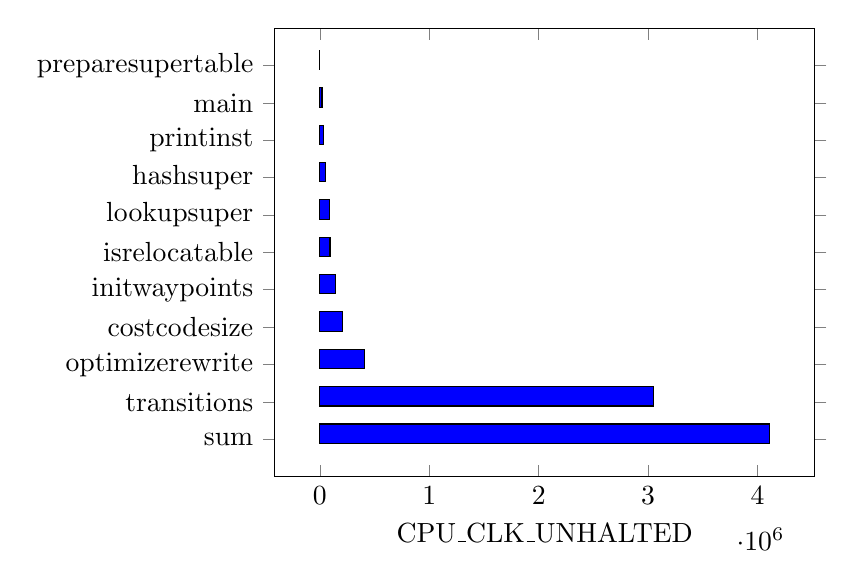
\begin{tikzpicture}
        \begin{axis}[   xbar,
                        symbolic y coords={sum,transitions,optimizerewrite,costcodesize,initwaypoints,isrelocatable,lookupsuper,hashsuper,printinst,main,preparesupertable},
                        xlabel=CPU\_CLK\_UNHALTED,
                        bar width=7pt,
                        bar shift=2pt,
                        ytick=data,
                        point meta=x * 10^7
                    ]
            \addplot+[draw=black, fill=blue] 
            coordinates {
                (3050495,transitions)
                (410243,optimizerewrite)
                (205597,costcodesize)
                (145182,initwaypoints)
                (93162,isrelocatable)
                (92836,lookupsuper)
                (55595,hashsuper)
                (34782,printinst)
                (20346,main)
                (676,preparesupertable)
                (4108914,sum)
            };
        \end{axis}
    \end{tikzpicture}
\end{frame}

\begin{frame}
    \frametitle{Ask not what you can do for your compiler}
    \begin{center} ... ask your compiler what he can do for you.
    \end{center}
\end{frame}

\begin{frame}
    \frametitle{Ask not what you can do for your compiler}
    \begin{itemize}
        \item -O3 statt -O0
        \item mass inlining
        \item unrolling
    \end{itemize}
\end{frame}

\begin{frame}
    \frametitle{Ask not what you can do for your compiler}
    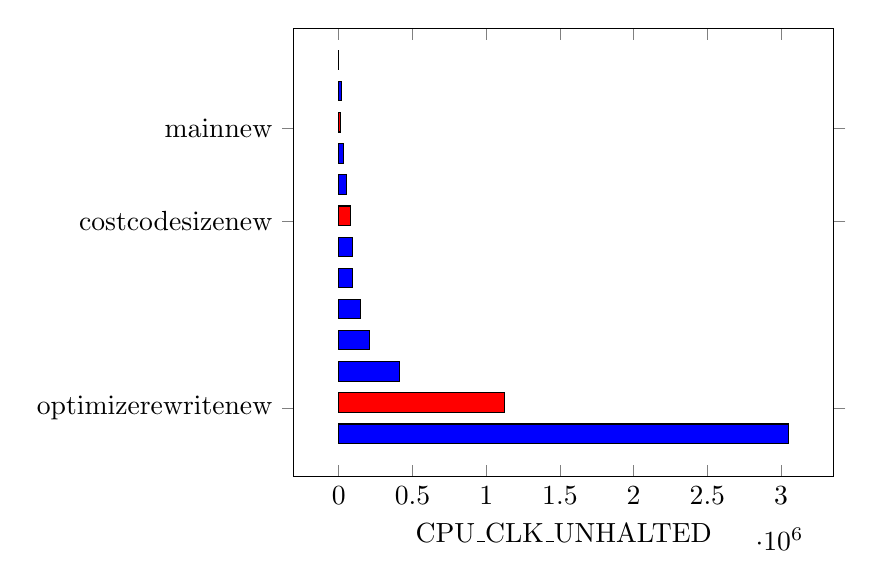
\begin{tikzpicture}
        \begin{axis}[   xbar,
                        symbolic y coords={transitions,optimizerewritenew, optimizerewrite,costcodesize,initwaypoints,isrelocatable,lookupsuper,
                                            costcodesizenew,hashsuper,printinst, mainnew, main, preparesupertable},
                        xlabel=CPU\_CLK\_UNHALTED,
                        bar width=7pt,
                        bar shift=2pt,
                        ytick=data,
                        point meta=x * 10^7
                    ]
            \addplot+[draw=black, fill=red] 
            coordinates {
                (1121706,optimizerewritenew)
                (78016,costcodesizenew)
                (11296,mainnew)
            };

            \addplot+[draw=black, fill=blue] 
            coordinates {
                (3050495,transitions)
                (410243,optimizerewrite)
                (205597,costcodesize)
                (145182,initwaypoints)
                (93162,isrelocatable)
                (92836,lookupsuper)
                (55595,hashsuper)
                (34782,printinst)
                (20346,main)
                (676,preparesupertable)
            };
        \end{axis}
    \end{tikzpicture}
\end{frame}

\begin{frame}
    \frametitle{Ask not what you can do for your compiler}
    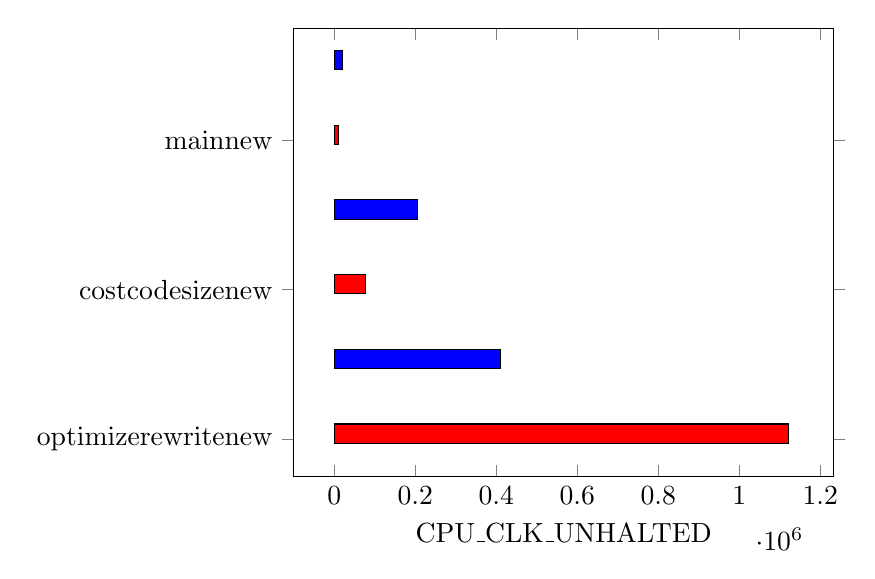
\begin{tikzpicture}
        \begin{axis}[   xbar,
                        symbolic y coords={optimizerewritenew, optimizerewrite, costcodesizenew, costcodesize, mainnew, main},
                        xlabel=CPU\_CLK\_UNHALTED,
                        bar width=7pt,
                        bar shift=2pt,
                        ytick=data
                    ]
            \addplot+[draw=black, fill=red] 
            coordinates {
                (1121706,optimizerewritenew)
                (78016,costcodesizenew)
                (11296,mainnew)
            };

            \addplot+[draw=black, fill=blue] 
            coordinates {
                (410243,optimizerewrite)
                (205597,costcodesize)
                (20346,main)
            };
        \end{axis}
    \end{tikzpicture}
\end{frame}

\begin{frame}
    \frametitle{Ask not what you can do for your compiler}
    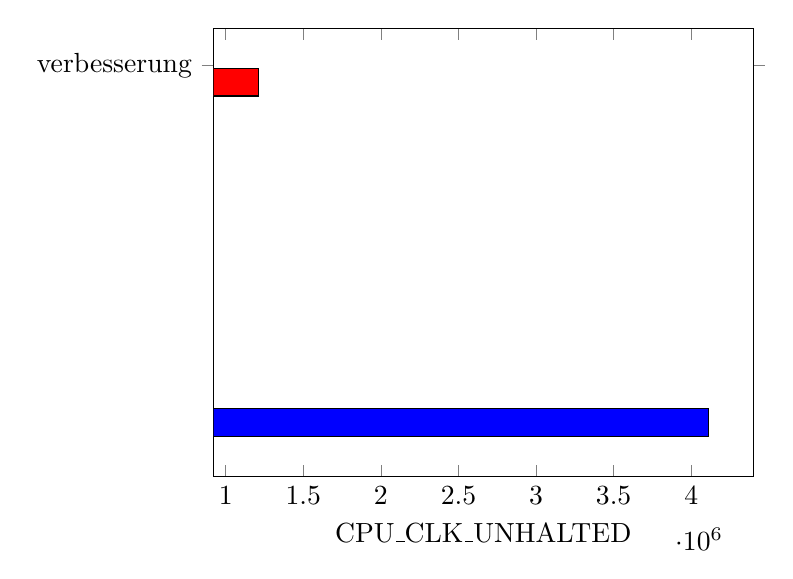
\begin{tikzpicture}
        \begin{axis}[   xbar,
                        symbolic y coords={ursprung, verbesserung},
                        xlabel=CPU\_CLK\_UNHALTED,
                        ytick=data
                    ]
            \addplot[draw=black, fill=red] 
            coordinates {
                (1211018,verbesserung)
            };

            \addplot[draw=black, fill=blue] 
            coordinates {
                (4108914,ursprung)
            };
        \end{axis}
    \end{tikzpicture}
\end{frame}

\begin{frame}
    \frametitle{Ask not what you can do for your compiler}
    \begin{center} ... but don't ask too much of him.
    \end{center}
\end{frame}

\begin{frame}
    \frametitle{Ask not what you can do for your compiler}
    \begin{itemize}
        \item -funroll-loops
    \end{itemize}
\end{frame}

\begin{frame}
    \frametitle{Ask not what you can do for your compiler}
    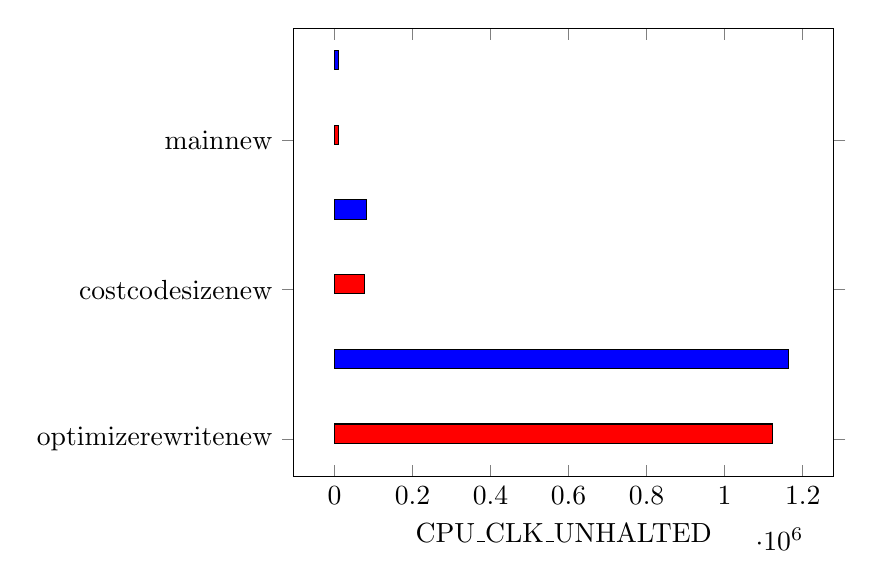
\begin{tikzpicture}
        \begin{axis}[   xbar,
                        symbolic y coords={optimizerewritenew, optimizerewrite, costcodesizenew, costcodesize, mainnew, main},
                        xlabel=CPU\_CLK\_UNHALTED,
                        bar width=7pt,
                        bar shift=2pt,
                        ytick=data
                    ]
            \addplot+[draw=black, fill=red] 
            coordinates {
                (1121706,optimizerewritenew)
                (78016,costcodesizenew)
                (11296,mainnew)
            };

            \addplot+[draw=black, fill=blue] 
            coordinates {
                (1163755,optimizerewrite)
                (80994,costcodesize)
                (11166,main)
            };
        \end{axis}
    \end{tikzpicture}
\end{frame}

\begin{frame}
    \frametitle{Lets actually do something}
    \begin{itemize}
        \item ersetze ss\_cost durch cost\_codesize
        \item costcodesize verschwindet komplett
        \item main und optimize rewrite marginal besser
    \end{itemize}
\end{frame}

\begin{frame}
    \frametitle{Lets actually do something}
    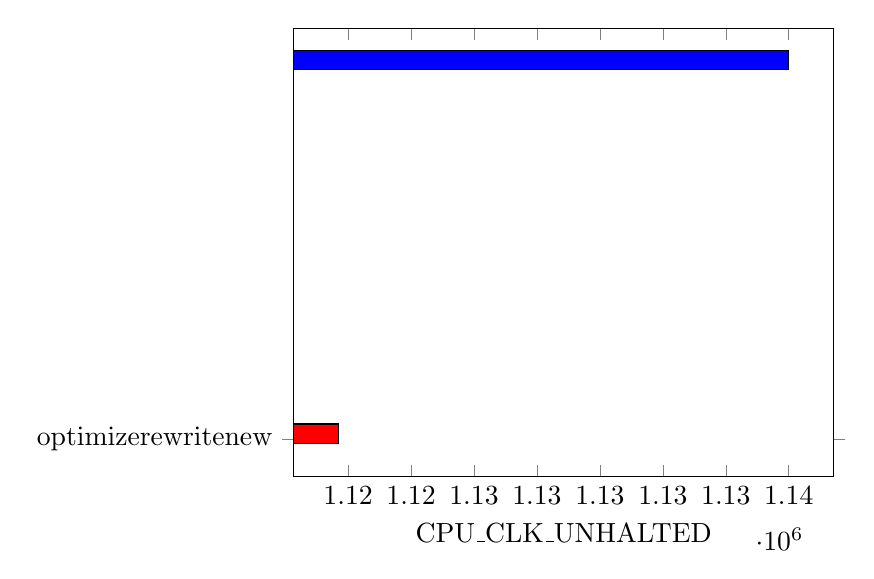
\begin{tikzpicture}
        \begin{axis}[   xbar,
                        symbolic y coords={optimizerewritenew, optimizerewrite},
                        xlabel=CPU\_CLK\_UNHALTED,
                        bar width=7pt,
                        bar shift=2pt,
                        ytick=data
                    ]
            \addplot+[draw=black, fill=red] 
            coordinates {
                (1121706,optimizerewritenew)
            };

            \addplot+[draw=black, fill=blue] 
            coordinates {
                (1135993,optimizerewrite)
            };
        \end{axis}
    \end{tikzpicture}
\end{frame}

\begin{frame}
    \frametitle{Lets actually do something}
    \begin{itemize}
        \item Verbesserung main Schleife
    \end{itemize}
\end{frame}

\begin{frame}
    \frametitle{Lets actually do something}
    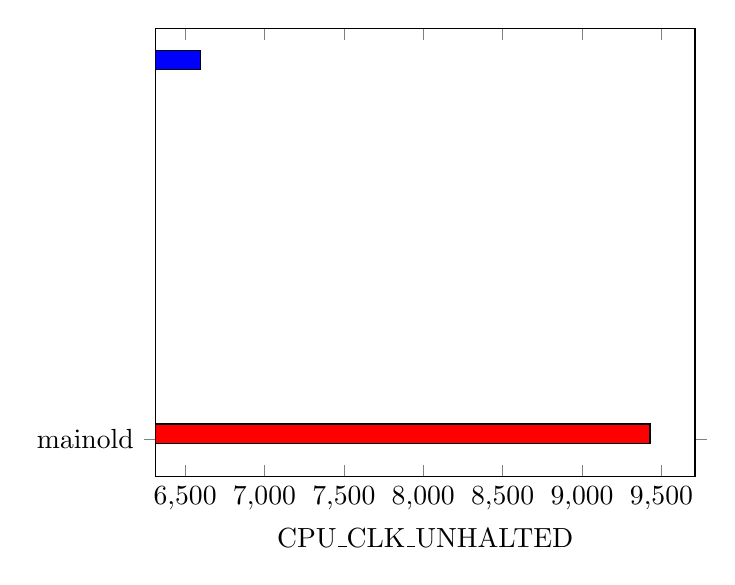
\begin{tikzpicture}
        \begin{axis}[   xbar,
                        symbolic y coords={mainold, mainnew},
                        xlabel=CPU\_CLK\_UNHALTED,
                        bar width=7pt,
                        bar shift=2pt,
                        ytick=data
                    ]
            \addplot+[draw=black, fill=red] 
            coordinates {
                (9428,mainold)
            };

            \addplot+[draw=black, fill=blue] 
            coordinates {
                (6596,mainnew)
            };
        \end{axis}
    \end{tikzpicture}
\end{frame}

\begin{frame}
    \url{http://leto.net/docs/C-optimization.php\#Compute-bound}
    \url{http://people.redhat.com/drepper/cpumemory.pdf}
    \url{http://www.fefe.de/dietlibc/diet.pdf}
    \url{http://www.fefe.de/know-your-compiler.pdf}
\end{frame}

\end{document}
